\chapter{Dynamic Obstacle Avoidance}
\label{chp:4-obstacle}

\par In this chapter, we use an external depth sensor to create a real time collision avoidance system. We start by describing how the sensor information is processed in order to detect obstacles in the environment. Then, from the identified obstacles we explain how they are segmented and the distances they present to the robot. Afterwards, we outline how an attraction and repulsion vectors are created and used to generate a final velocity vector which the robot will use to avoid dynamic obstacles when executing predefined static trajectories. Finally, we describe a software architecture that implements the previous models in real time.






\section{Obstacle Detection}
\label{section:obstacle-detection}

% Introduction on obstacle detection
\par In order for a robot to avoid obstacles while in motion, an external vision sensor is used to capture the shared workspace and send information to the system about the robot surroundings. In this Dissertation, an \ac{rgbd} camera will be used for this purpose. It gives the system depth information on its \ac{fov}, referenced to itself. The first step in this endeavour is to spatially and dynamically reference the camera to the robot through hand eye calibration. 



\subsection{Hand Eye Calibration}

% Application of hand eye calibration 
\par This process is able to generate an accurate transform from the robot base frame to the sensor frame. In this proposal, a fiducial marker based on the ARuco library \cite{aruco} is fixed on the robot \ac{eef}. Then, using the \textit{easy\_handeye} \ac{ros} package, a set of translations and rotations are performed at the \ac{eef} level. In each movement, a sample composed of the \ac{eef} pose and the ARuco pose, identified by the sensor, is captured. A total of 3 translations and 6 rotations are performed in each axis, making a total of 27 samples. When the sampling is finished, the \textit{easy\_handeye} compute service is called and a static transform is obtained, which is both locally saved and published in the \ac{ros} environment.

% TODO 2 fotos aqui, uma real, outra do RViz



\subsection{Robot Segmentation}

% Necessity of robot self identification
\par Since the camera will be sensing the shared workspace, there will be multiple scenarios where the robot will enter its \ac{fov}. Robot segmentation consists on a method to identify which points of the point cloud belong to the robot structure, in order to differentiate obstacles from the robot when both of them are in the sensor \ac{fov}.

% Build a skeleton of the robot and identify points belonging to it
\par The technique developed in this work starts by building a skeleton model of the robot, starting with the location of its links. The position of these links, defined in the robot \ac{urdf} present in its \ac{ros} driver, does not match the real position of the robot arms and wrists, therefore, from these links, a set of points are created representing the start and end of each real link. Using this set of points and a minimum distance constant, the skeleton model is created based on \autoref{code:robot_skeleton}. The difference between the links defined in the robot \ac{urdf} and the points created can be seen in \autoref{fig:links_to_points}.

\begin{listing}[h]
    \centering
    \begin{minted}{python}

    def ur10eSkeleton(min_dist = 0.05):
        skeleton = []
        links = ROS.TransformLibrary.getLinks()
        points = obtainPoints(links)

        for point in points:  
            skeleton.append(point)
            distance = point.distance(point.next())
            num_skeleton_points = distance / min_dist
            increment = (point - point.next()) / num_skeleton_points

            for i in range(num_skeleton_points):
                skeleton.append(point + i * increment)

        return skeleton
    
    \end{minted}
\caption{Creation of a point based skeleton model of the robot}
\label{code:robot_skeleton}
\end{listing}

\begin{figure}[h]
    \centering
    \begin{subfigure}{.33\linewidth}
      \centering
      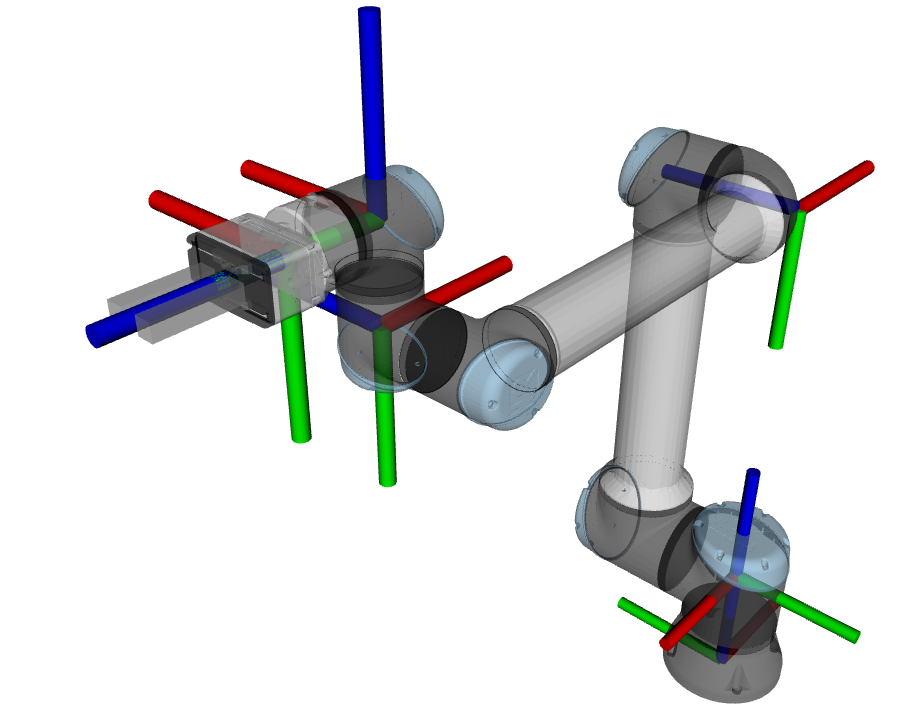
\includegraphics[width=.95\linewidth]{figs/chp4/self_ident_links.png}
    \end{subfigure}%
    \begin{subfigure}{.33\linewidth}
      \centering
      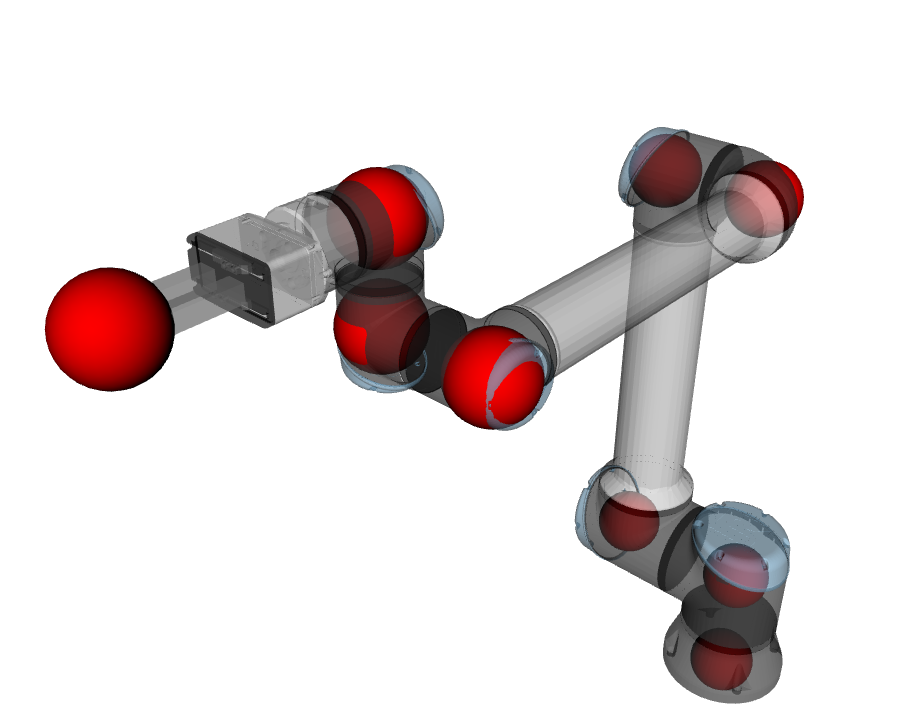
\includegraphics[width=.95\linewidth]{figs/chp4/self_ident_points.png}
    \end{subfigure}%
    \begin{subfigure}{.33\linewidth}
        \centering
        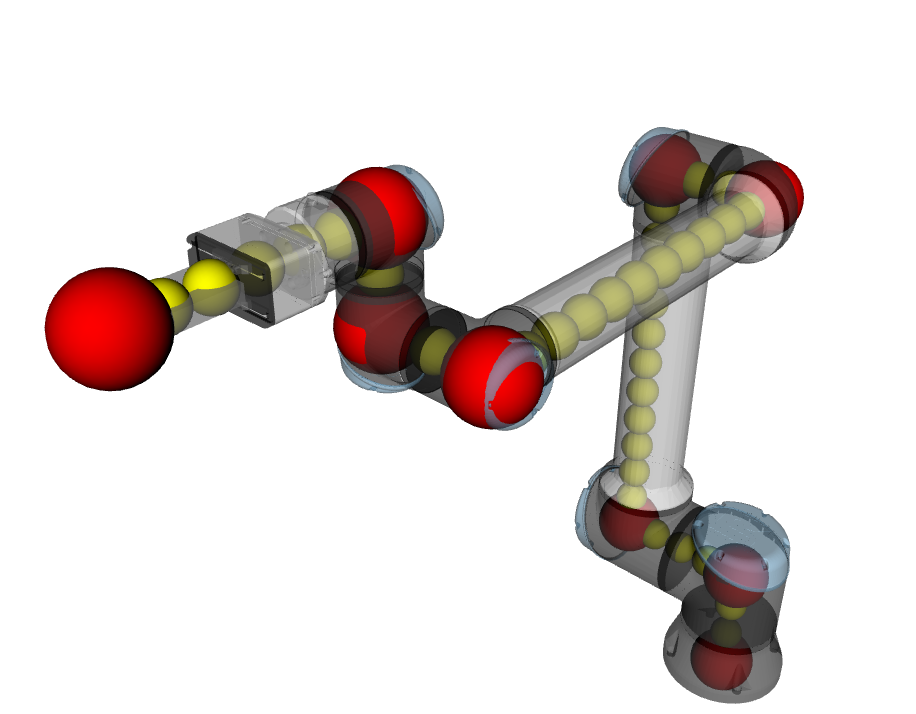
\includegraphics[width=.95\linewidth]{figs/chp4/self_ident_skeleton.png}
    \end{subfigure}
    \caption{Visual representation of the conversion from \ac{urdf} links to robot skeleton}
    \label{fig:links_to_points}
\end{figure}

% With the skeleton, the points on the point cloud belonging to the robot can be identified
\par From the resultant skeleton, any point from the point cloud that is closer to it than a predefined threshold, is considered belonging to the robot, therefore, not accounted for in the obstacle segmentation process. Also not accounted for, are points on the point cloud that are too far away from the robot. Based on a another distance constant, a \ac{roi} is created, and points that are further distant from the skeleton than it, are considered irrelevant. The final result of robot segmentation can be observed in \autoref{fig:self_ident_result}.

\begin{figure}[h]
    \centering
    \begin{subfigure}{.5\linewidth}
      \centering
      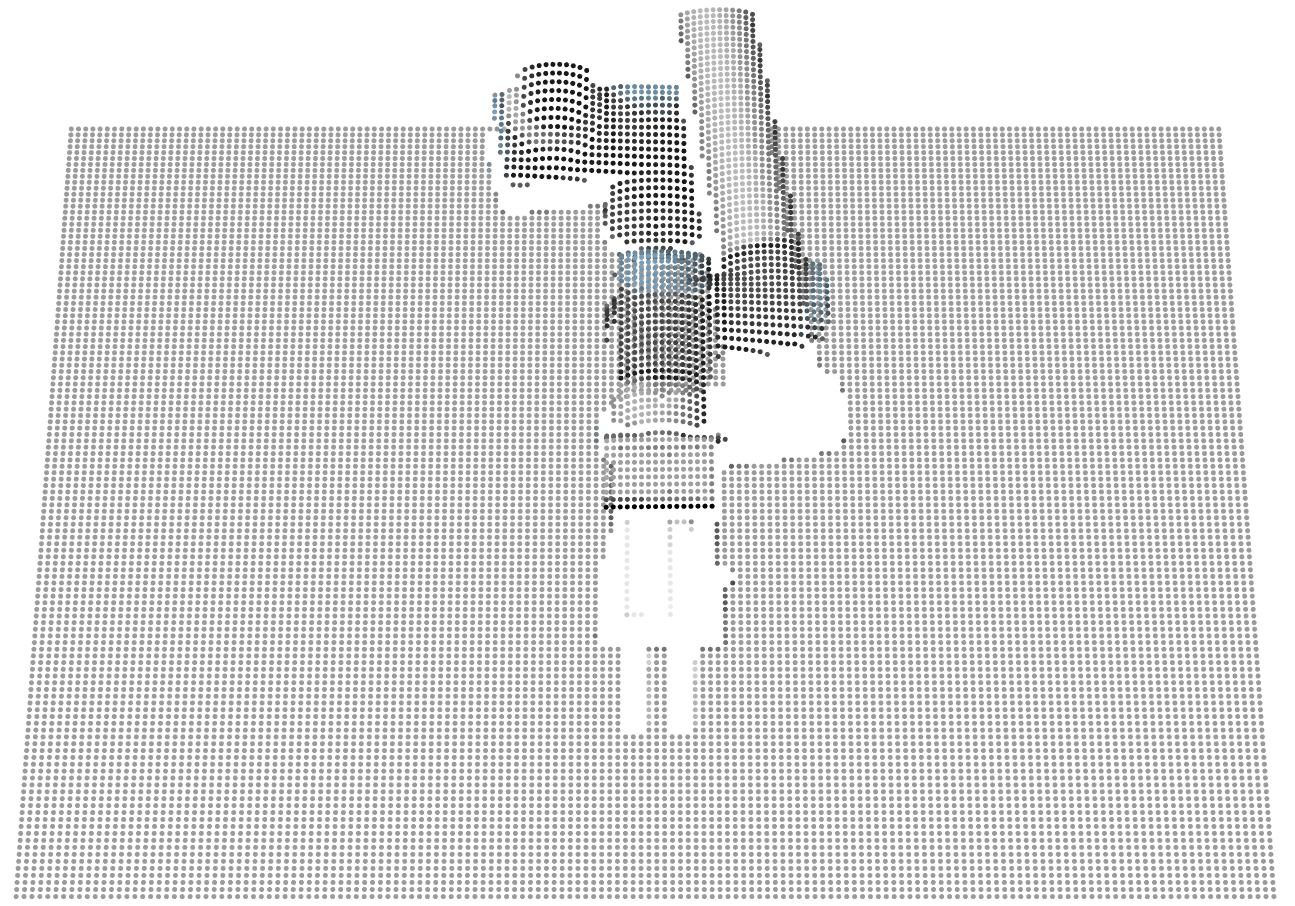
\includegraphics[width=.95\linewidth]{figs/chp4/cloud_before.png}
    \end{subfigure}%
    \begin{subfigure}{.5\linewidth}
      \centering
      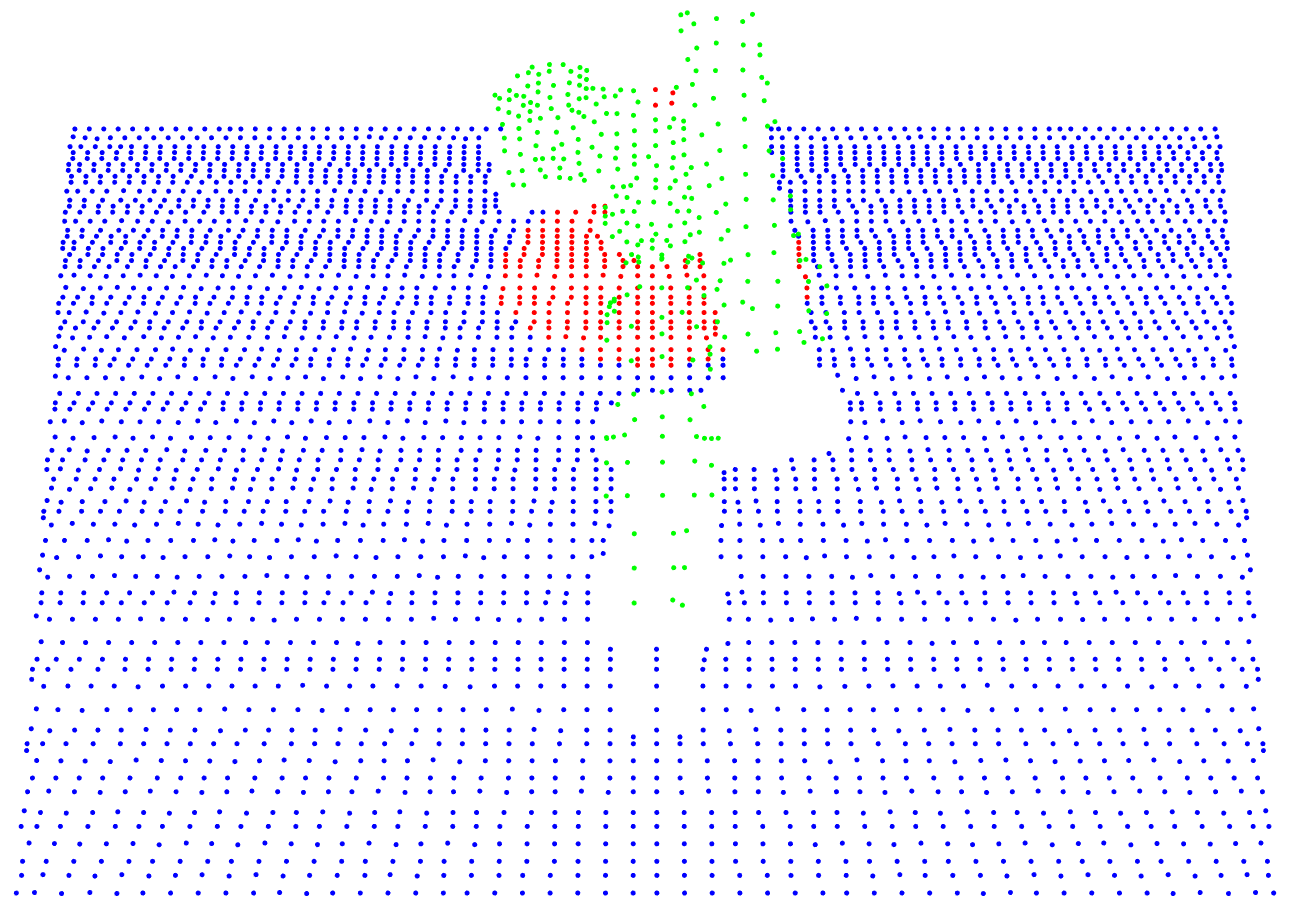
\includegraphics[width=.95\linewidth]{figs/chp4/cloud_after.png}
    \end{subfigure}
    \caption{Raw point cloud and categorized point cloud with \ac{roi}}
    \label{fig:self_ident_result}
\end{figure}



\subsection{Obstacle Segmentation}

% Categorization of the points with the ROI
\par Starting from the raw point cloud obtained from the sensor, each point is categorized. Points belonging to the robot, and points too distant from it are removed. Only points belonging to the \ac{roi}, if there are any, are considered obstacles, therefore, a new point cloud is created with these points.

% Application of CEC to the categorized point cloud
\par To this new point cloud, a clustering algorithm is applied in order to represent the point cloud in a set of small clusters, each one to be considered an obstacle. The algorithm applied is the \ac{cec}, which is a region growing algorithm based on the \ac{ece} algorithm. It has the advantage of allowing a customizable clustering condition and also classifying clusters as too small or too large, based on defined parameters. The parameters for the \ac{cec} implementation, used in this work, can be found in \autoref{tbl:cec_params}.

\begin{table}[h]
    \centering
    \begin{tabular}{|l|c|}
    \hline
    \textbf{Parameter} & \textbf{Value} \\ \hline
    Leaf Size & 0.3 \\ \hline
    Radius Search & 0.4 \\ \hline
    Cluster Tolerance & 0.5 \\ \hline
    Min Cluster Size & 5 \\ \hline
    Max Cluster Size & 90 \\ \hline
    Squared Distance & 0.001 \\ \hline
    \end{tabular}
    \caption{Internal parameters of the \ac{cec} algorithm}
    \label{tbl:cec_params}
\end{table}

% Results of the application of CEC
\par The result of this algorithm is a set of clusters and to each cluster, its closest point to the robot is calculated, achieving the obstacle collision point. \autoref{fig:obstacles} illustrates the obstacle detection final result, where 2 obstacles are present in the environment. One of them is outside the \ac{roi}, therefore ignored. The other, which is closer to the robot, is correctly identified.

\begin{figure}[h]
    \centering
    \begin{subfigure}{.5\linewidth}
      \centering
      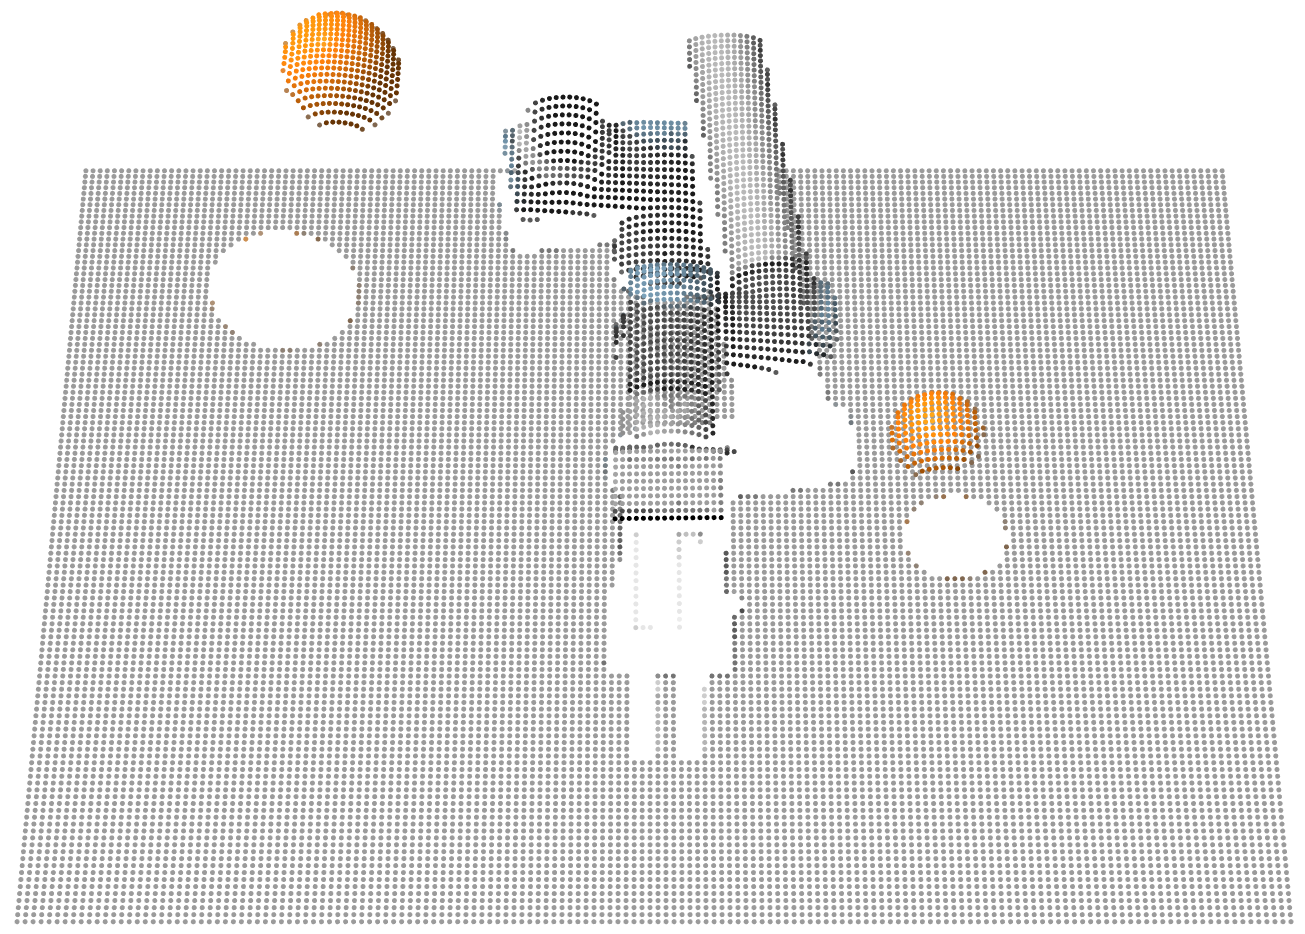
\includegraphics[width=.95\linewidth]{figs/chp4/obstacles_before.png}
    \end{subfigure}%
    \begin{subfigure}{.5\linewidth}
      \centering
      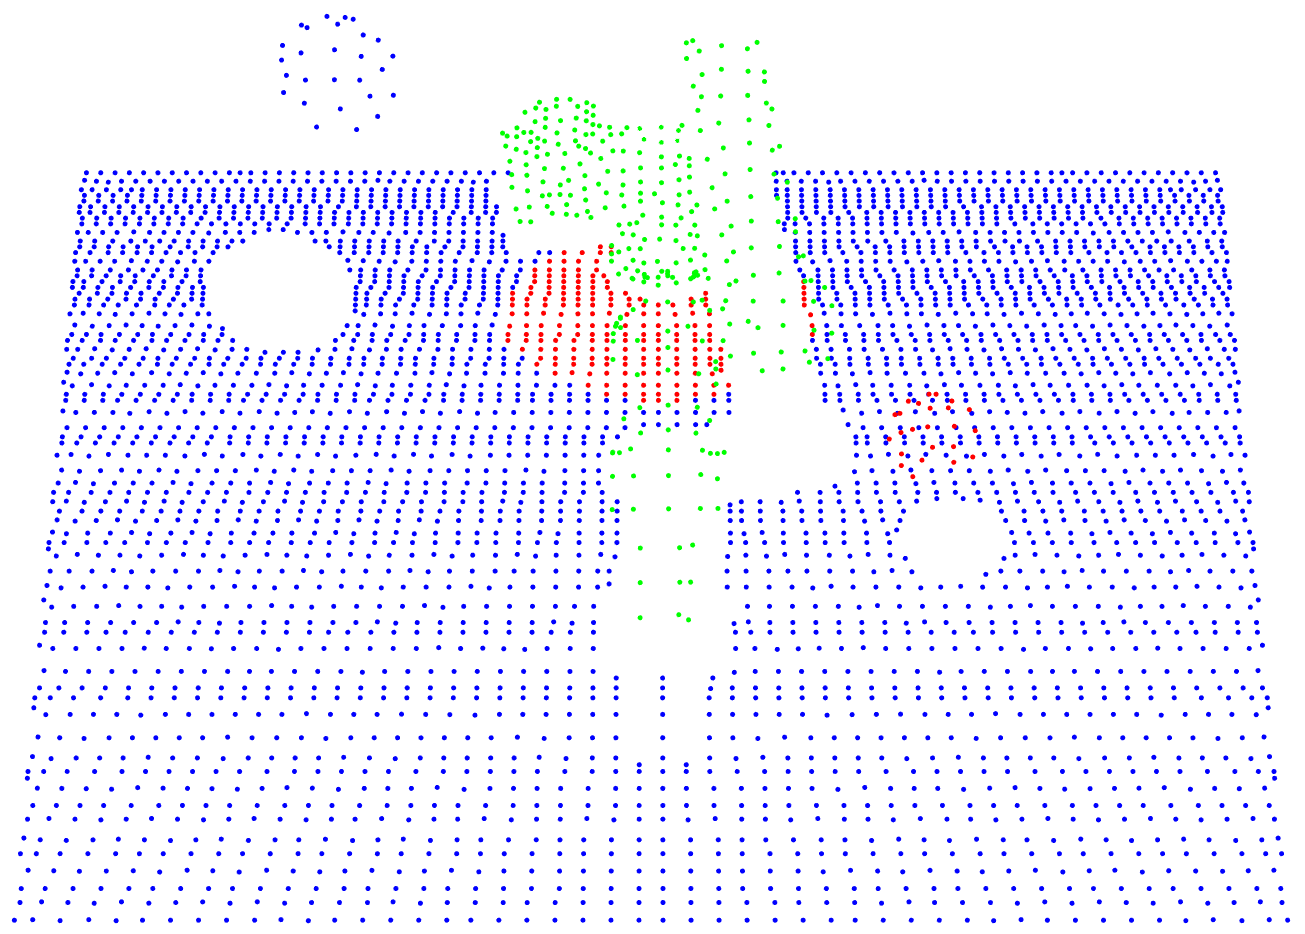
\includegraphics[width=.95\linewidth]{figs/chp4/obstacles_after.png}
    \end{subfigure}
    \caption{Final result of the obstacle segmentation algorithm}
    \label{fig:obstacles}
\end{figure}





\section{Artificial Potential Fields}
\label{section:pf-method}

% Introduction on APF
\par A well known method of dealing with real time collision avoidance on robotic manipulators is to treat the robot navigation as if it was a point in a potential field, and is called \ac{apf}. An \ac{apf} is the result of the sum of 2 fields. An attraction field, converging on the goal and a repulsion field created by obstacles in the environment. Within the final field, the robot can navigate successfully while avoiding the obstacles. Adapted to the context of robotic manipulators, the robot is in an imaginary vector field and its motion is the result of attraction forces, making the robot follow a predefined trajectory, and repulsion forces that repel it away from obstacles.



\subsection{Attraction}
\label{ssec:attraction}

% TODO Improve the generation and execution of offline trajectories

% Generation of an attraction vector based on an offline trajectory
\par The attraction force is what makes the robot move to its goal. In this work, this is done by generating a trajectory offline, and in real time make the robot follow the trajectory with cartesian space velocity commands.

% Generation of the offline trajectory
\par The first step is to generate an offline trajectory. A trajectory needs a start state and a goal state, and if no static obstacles are declared, the motion planner will generate an optimized trajectory based on those two inputs. Other factors might impact the final result but for the focus of this work, offline motion planning will not be discussed in detail. The trajectories generated with the MoveIt framework are arrays of joint positions, since it is designed to work with joint position controllers. In this work, the attraction and repulsion forces will be declared in cartesian space, therefore after obtaining the trajectory, all trajectory steps are converted to poses in cartesian space. This can be observed in the first subfigure of \autoref{fig:attraction}.

\begin{figure}[h]
    \centering
    \begin{subfigure}{.2\linewidth}
      \centering
      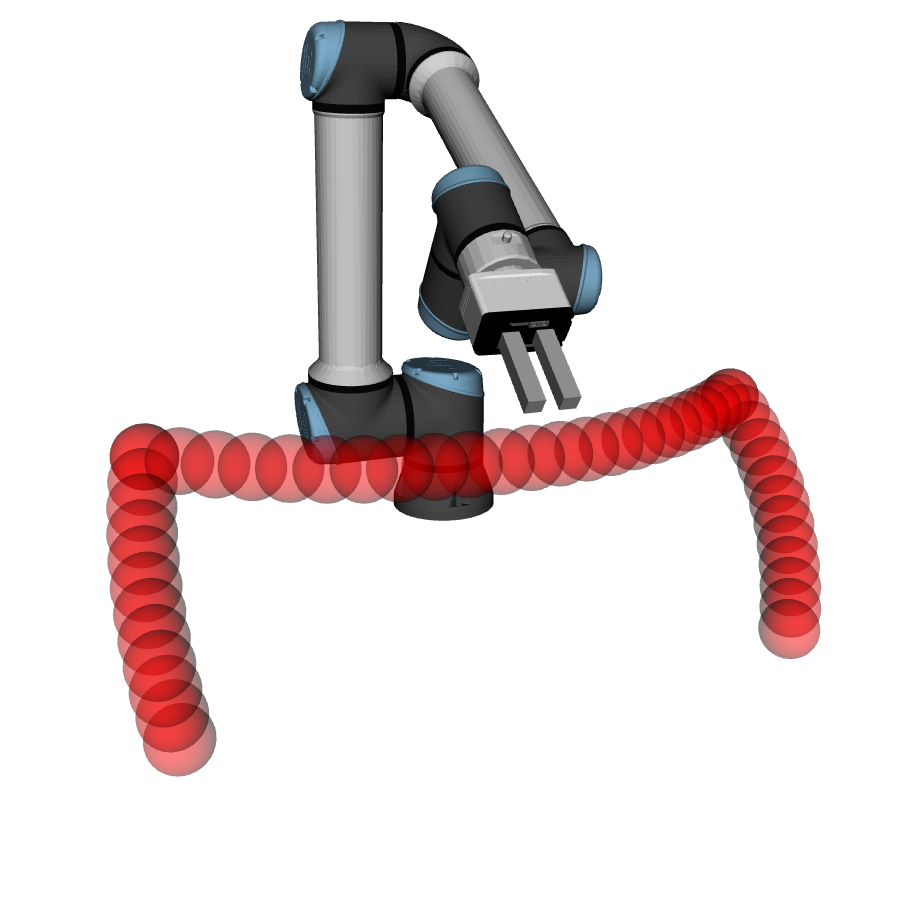
\includegraphics[width=\linewidth]{figs/chp4/trajectory_0.png}
    \end{subfigure}%
    \begin{subfigure}{.2\linewidth}
      \centering
      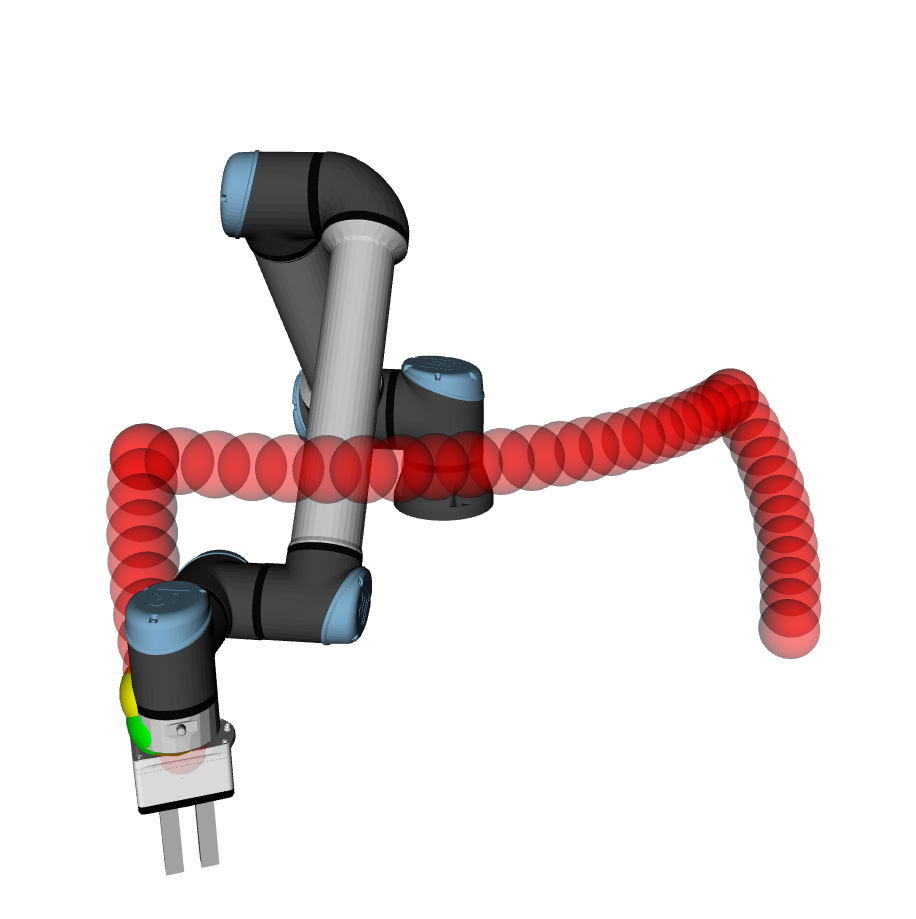
\includegraphics[width=\linewidth]{figs/chp4/trajectory_1.png}
    \end{subfigure}%
    \begin{subfigure}{.2\linewidth}
        \centering
        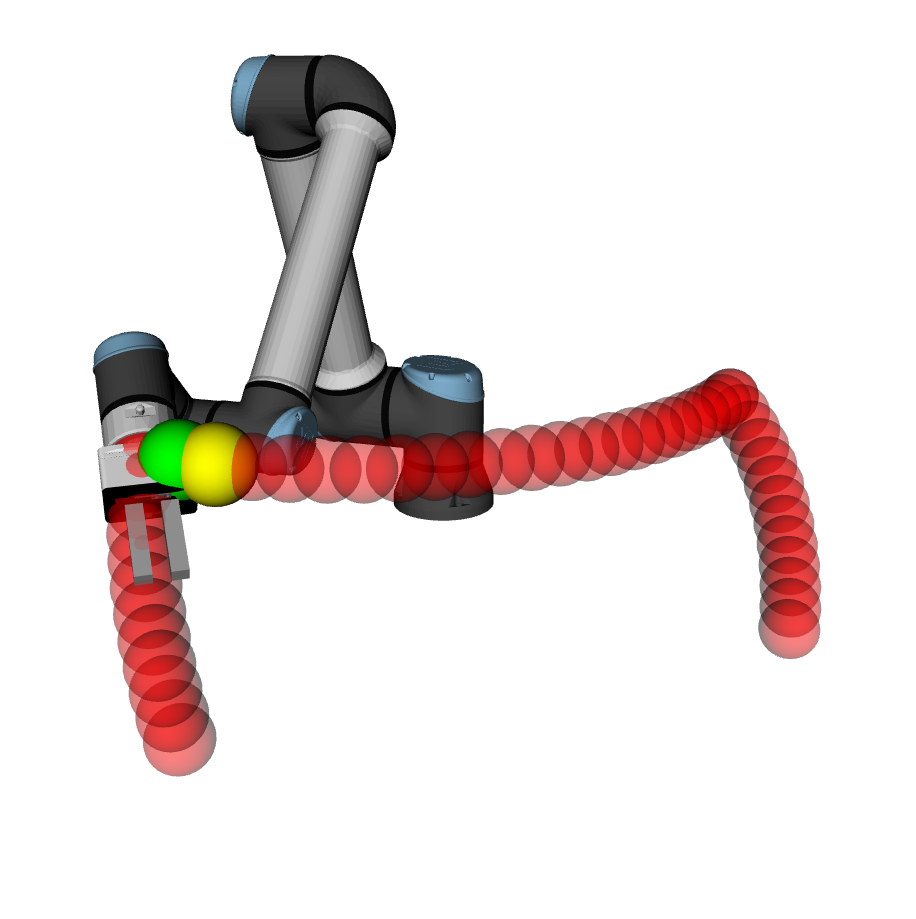
\includegraphics[width=\linewidth]{figs/chp4/trajectory_2.png}
    \end{subfigure}%
    \begin{subfigure}{.2\linewidth}
        \centering
        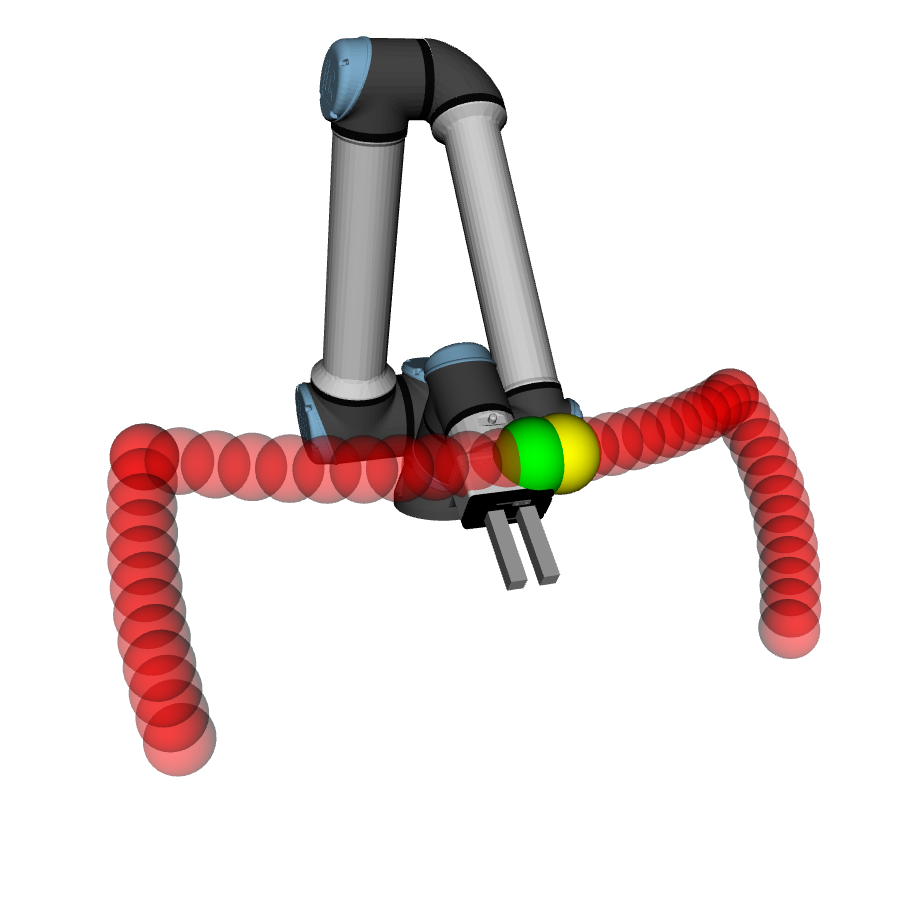
\includegraphics[width=\linewidth]{figs/chp4/trajectory_3.png}
    \end{subfigure}%
    \begin{subfigure}{.2\linewidth}
        \centering
        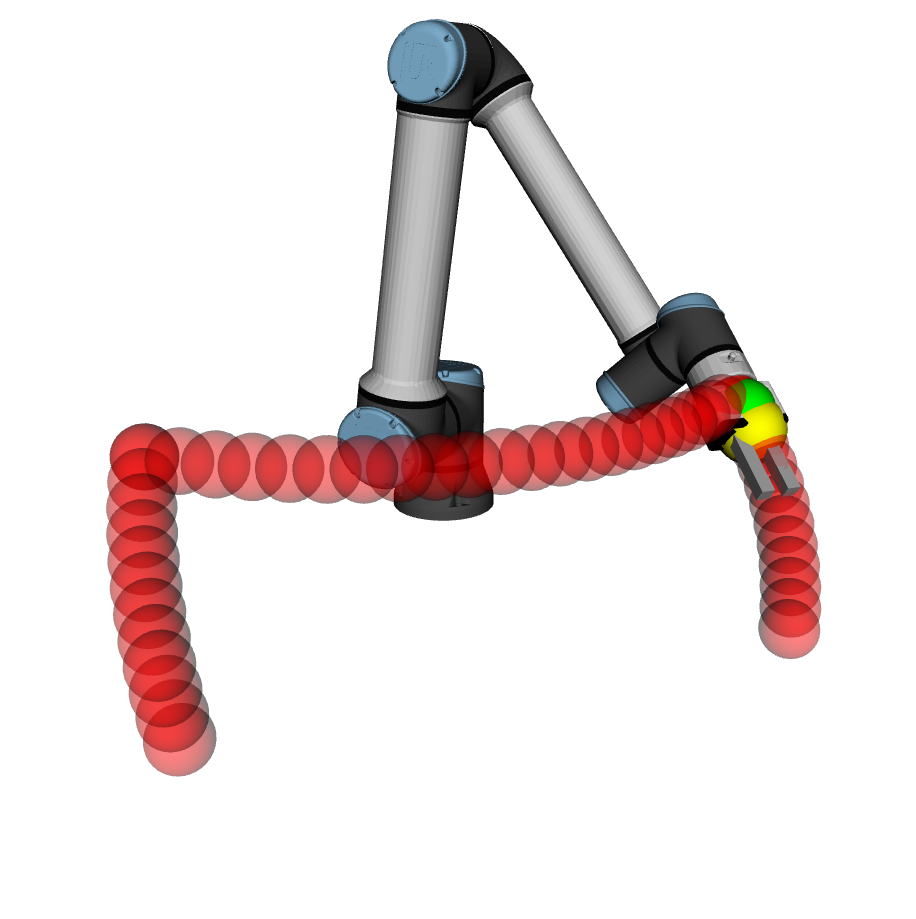
\includegraphics[width=\linewidth]{figs/chp4/trajectory_4.png}
    \end{subfigure}
    \caption{Trajectory execution with cartesian attraction vector}
    \label{fig:attraction}
\end{figure}

% Execution of the offline trajectory
\par After obtaining the set of poses, the robot will start executing the trajectory in its first point. For this initial position, the robot is moved with a joint position command. After the initial state, in a 500Hz loop a cartesian attraction vector, which is the difference between the current \ac{eef} position and the next point in the trajectory, is obtained with \autoref{eq:attraction}.

% TODO Review this equation
\begin{equation}
    \vec{\mathbf{Att}}=P_{goal}\cdot {T_e^b}^{-1}
    \label{eq:attraction}
\end{equation}

\noindent Where $\mathbf{P_{goal}}$ is the pose of the goal point in the trajectory and $\mathbf{T_e^b}$ a transformation from the base frame to the \ac{eef} frame. $\vec{\mathbf{Att}}$ is obtained in the form of a pose object. The position part will be the linear velocity and the orientation part will be the angular velocity. This vector is constantly being calculated based on the monitoring of the \ac{eef} and the calculation of the new goal.



\subsection{Repulsion}
\label{ssec:repulsion}

% Creation of a repulsion vector based on an array of obstacles
\par The obstacle segmentation algorithm produces an array of obstacles. Each obstacle is defined by its pose. The repulsion vector is calculated using this pose and the \ac{eef} pose, since its the most likely part of the robot to colide with obstacles. Within the array of obstacles, the closest to the \ac{eef} is selected. A repulsion vector is created with this obstacle based on how distant it is to the \ac{eef} with \autoref{eq:repulsion}.

\begin{equation}
    \vec{\mathbf{Rep}} = \frac{P_{eef}-P_{obs}}{\mid\mid P_{eef}-P_{obs} \mid\mid}\cdot\frac{max_d-(d-min_d)}{max_d} 
    \label{eq:repulsion}
\end{equation}

\noindent Where $\mathbf{P_{eef}}$ is the \ac{eef} pose, $\mathbf{P_{obs}}$ is the obstacle pose, $\mathbf{d}$ is the distance between the \ac{eef} and the obstacle, and $\mathbf{max_d}$ and $\mathbf{min_d}$ are maximum and minimum distance constants, respectively. $\vec{\mathbf{Rep}}$ is obtained in the form of a linear vector since, in the repulsion vector calculation, angular velocity is not accounted for. The first part of this equation represents a unit vector with the direction of the obstacle, and the second part can be seen as a repulsion factor, which consists on a linear function that ranges from $\frac{min_d}{max_d}$ to 1. This factor causes the magnitude of the repulsion vector to increase as the distance to the obstacle decreases.



\subsection{Controller}

% Creation of a final normalized vector to give the robot its motion
\par The \ac{apf} controller sums the forces from the two components. In this work, the chosen approach is to create a final cartesian velocity vector, taking as inputs the two forces previously explained. The final velocity for the robot \ac{eef} is calculated with \autoref{eq:potential_field}.

\begin{equation}
    \vec{\mathbf{V_{eef}}}=(1\:-\mid\mid\vec{Rep}\mid\mid)\cdot\vec{Att}\:+\mid\mid\vec{Rep}\mid\mid\cdot \vec{Rep}
    \label{eq:potential_field}
\end{equation}

\par This way, when there are no obstacles, $\mid\mid\vec{\mathbf{Rep}}\mid\mid\mathbf{=0}$, therefore, $\vec{\mathbf{V_{eef}}}=\vec{\mathbf{Att}}$. When obstacles do exist, the controller will give priority to the repulsion vector as is starts to grow, since as seen in \autoref{ssec:repulsion}, the repulsion vector norm increases as the distance to obstacles decreases.





\section{Real Time Obstacle Avoidance}
\label{sec:obstacle-architecture}

% TODO Improve this section with further implementation details

% ROS Architecture for obstacle avoidance
\par Similarly to the correction and compensation of \ac{ft}, a group of \ac{ros} nodes was developed and orchestrated in order to give the robot the ability to avoid dynamic obstacles while in motion and in real time. \autoref{fig:ros_obstacle_arch} demonstrates how those nodes are arranged.

\begin{figure}[h]
    \centering
    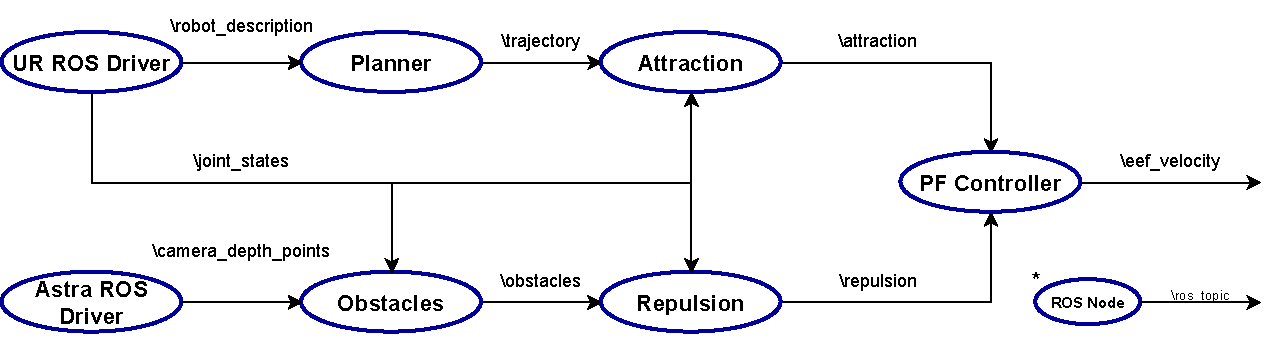
\includegraphics[width=\linewidth]{figs/chp4/ros_obstacle_arch.pdf}
    \caption{\ac{ros} architecture of the obstacle avoidance in real time}
    \label{fig:ros_obstacle_arch}
\end{figure}

% Explanation of the various nodes
\par The attraction component starts at the Planner node, which uses the MoveIt motion planning interface to generate trajectories. It obtains the \ac{ur10e} description from its driver and with a move group object plans and publishes robot trajectories. The attraction node listens to the trajectories published by the Planner node and acts according to what was described in \autoref{ssec:attraction}. On the repulsion side, the Obstacles node listens to the point clouds published by the sensor driver and publishes an array with obstacle information. From that information, the Repulsion node publishes the repulsion vector, according with \autoref{ssec:repulsion}. Finally the \ac{apf} Controller node joins the attraction and repulsion vectors, publishing the final \ac{eef} velocity vector.

\begin{figure}[h]
    \centering
    \begin{subfigure}{.5\linewidth}
      \centering
      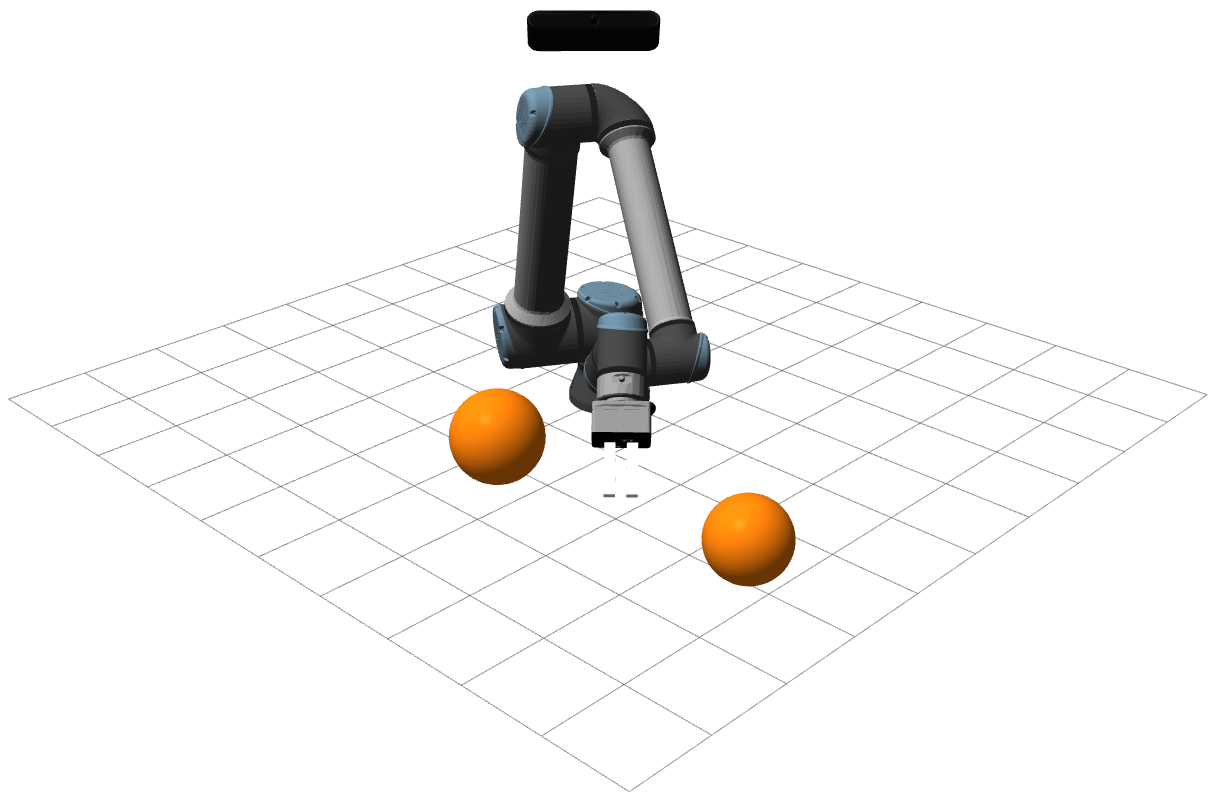
\includegraphics[width=\linewidth]{figs/chp4/col_avoid_gazebo_mid.png}
    \end{subfigure}%
    \begin{subfigure}{.5\linewidth}
      \centering
      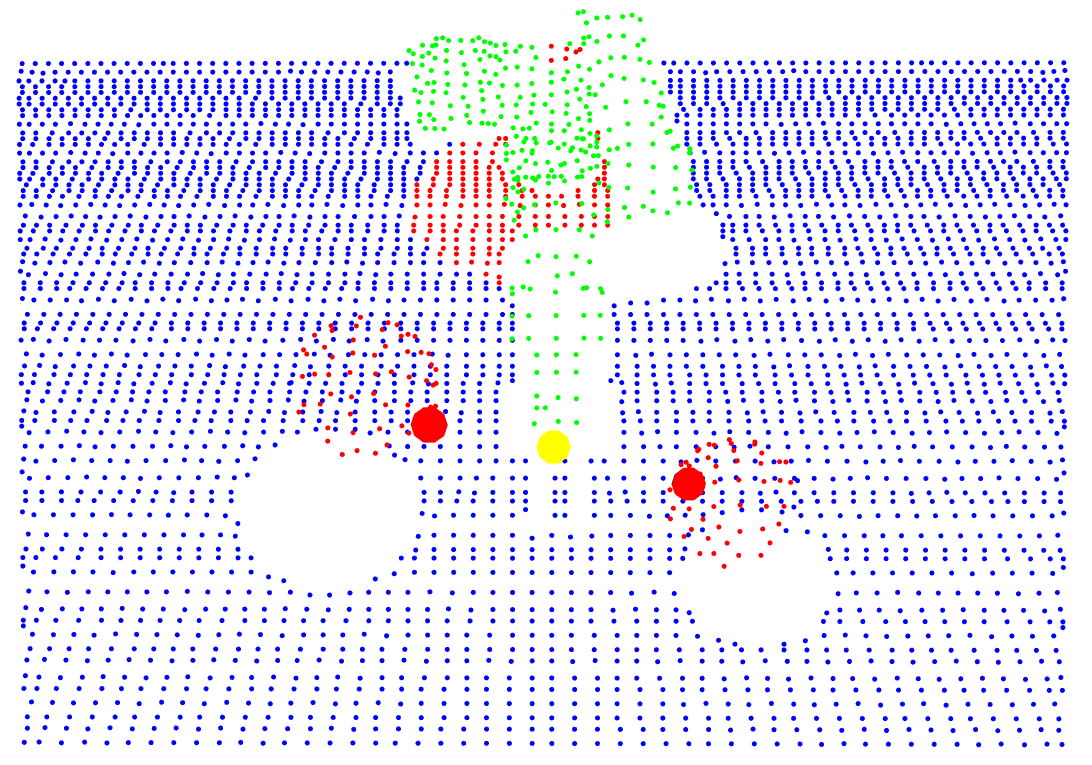
\includegraphics[width=0.9\linewidth]{figs/chp4/col_avoid_pcl.png}
    \end{subfigure}
    \caption{Collision avoidance setup in the Gazebo simulator}
    \label{fig:gazebo}
\end{figure}

% Testing of the architecture with the execution of an offline trajectory with obstacles
\par A testing environment was built in the Gazebo simulator. The \ac{ur10e} was placed in the center of the world, an RGBD camera was placed on top of it, overlooking an area considered the shared environment, where 2 sphere obstacles were spawned. This setup can be seen in \autoref{fig:gazebo}. A trajectory was created that would intentionally colide with these obstacles. 

\begin{figure}[h]
    \centering
    \begin{subfigure}{.50\linewidth}
      \centering
      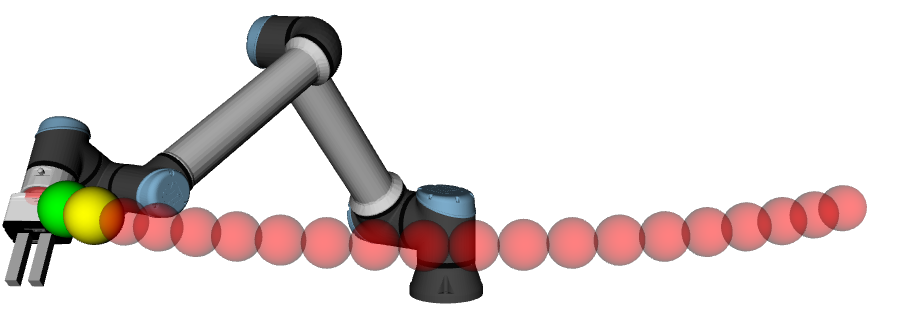
\includegraphics[width=\linewidth]{figs/chp4/col_avoid_start.png}
    \end{subfigure}%
    \begin{subfigure}{.50\linewidth}
        \centering
        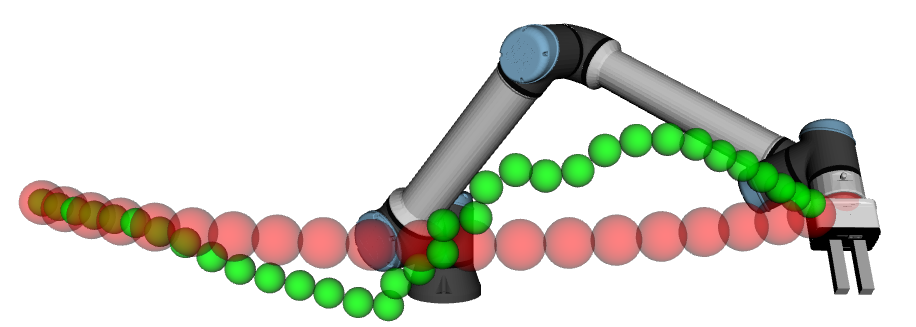
\includegraphics[width=\linewidth]{figs/chp4/col_avoid_end.png}
    \end{subfigure}
    \caption{Collision avoidance offline and final trajectory}
    \label{fig:colision_avoidance}
\end{figure}

% Final remark on the final trajectory obtained
\par The offline trajectory and the final trajectory that the robot performed with the collision avoidance nodes enabled can be seen in \autoref{fig:colision_avoidance}. Further details on the performance of this architecture and details on the implementation on a real scenario will be outlined in \autoref{sec:colision_tests}.
